Um das Game mit dem Arduino besser steuern zu können, haben wir einen Joystick gedruckt um das Benutzerfeeling zu verbessern.

\begin{figure}[H]
    \begin{center}
      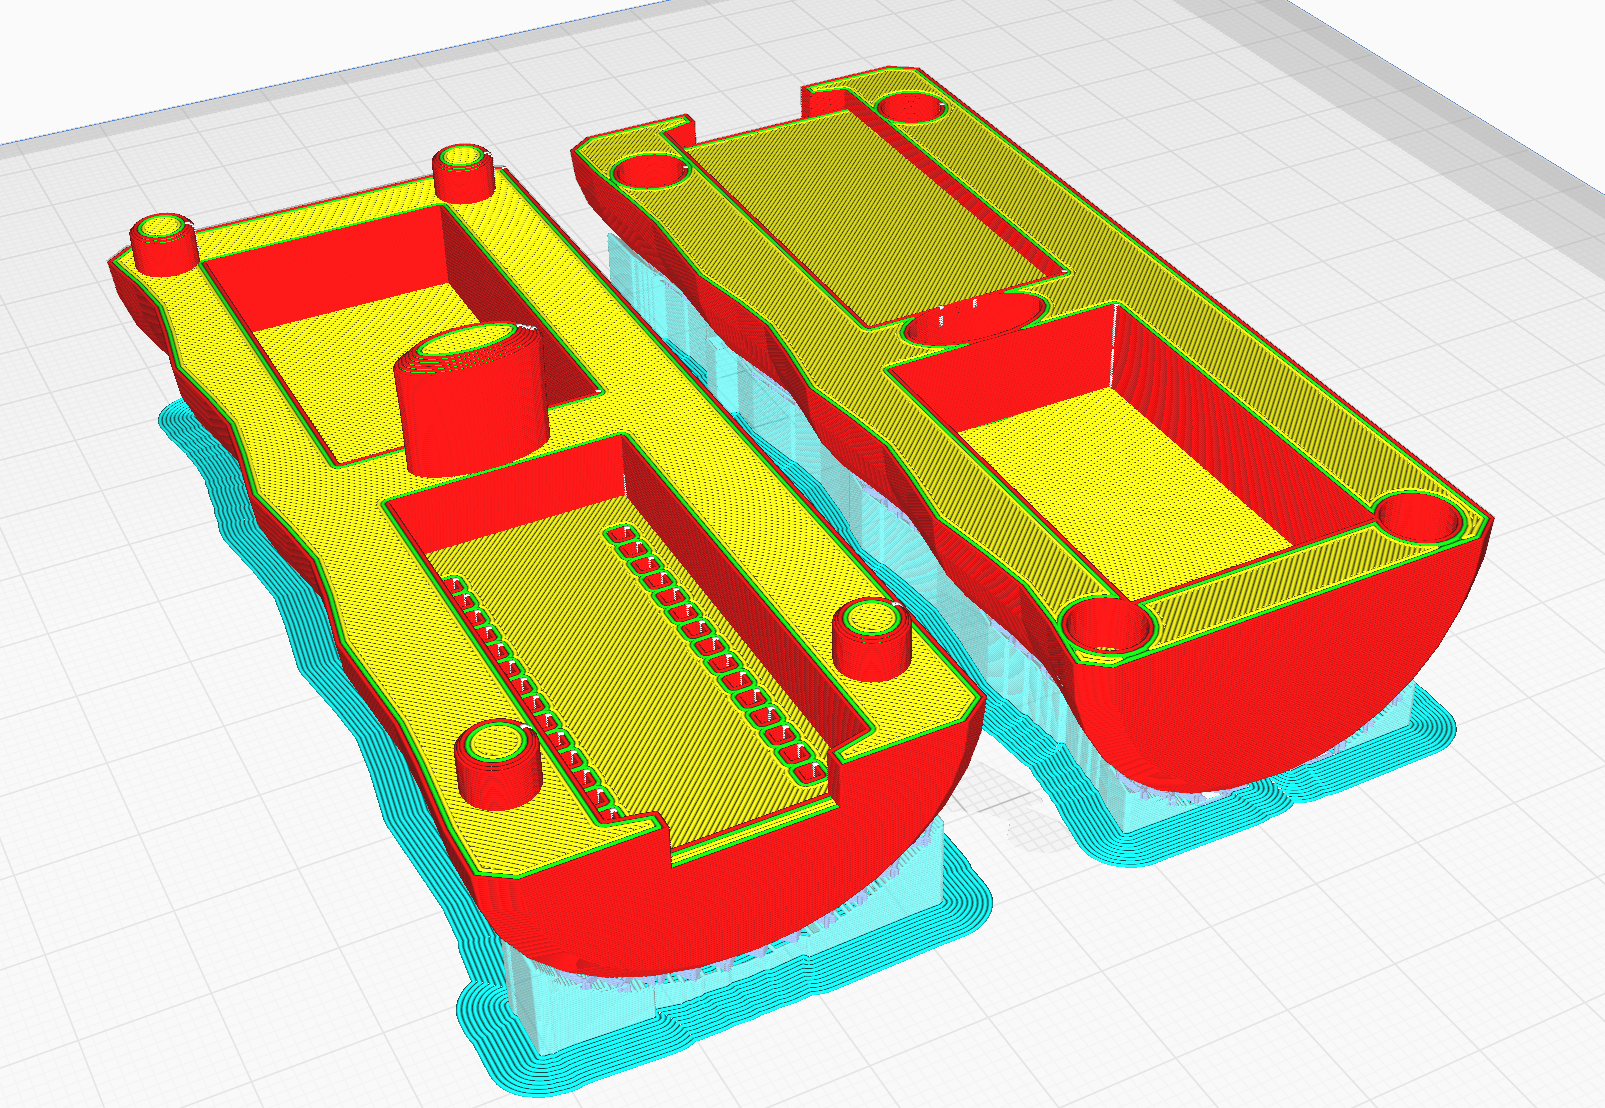
\includegraphics[width=0.7\linewidth]{content/images/Joystick_3D-Print_Slicer.jpg}
      \caption{3D Druck Slicer}
    \end{center}
  \end{figure}

\begin{minipage}[l]{0.49\textwidth}
  \begin{figure}[H]
    \begin{center}
      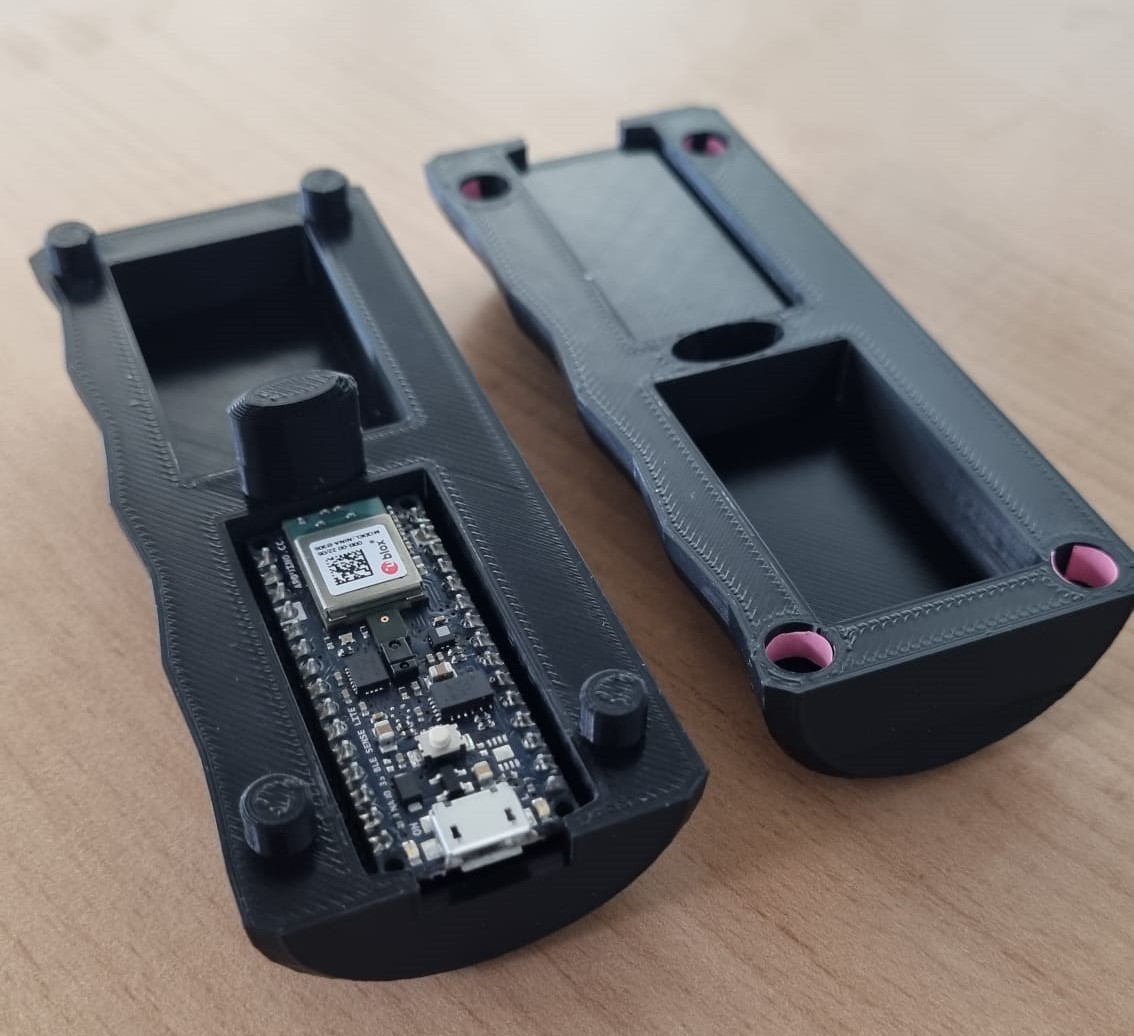
\includegraphics[width=1\linewidth]{content/images/3DPrint_open.jpeg}
      \caption{3D Druck geöffnet}
    \end{center}
  \end{figure}
\end{minipage}
\begin{minipage}[r]{0.5\textwidth}
  \begin{figure}[H]
    \begin{center}
      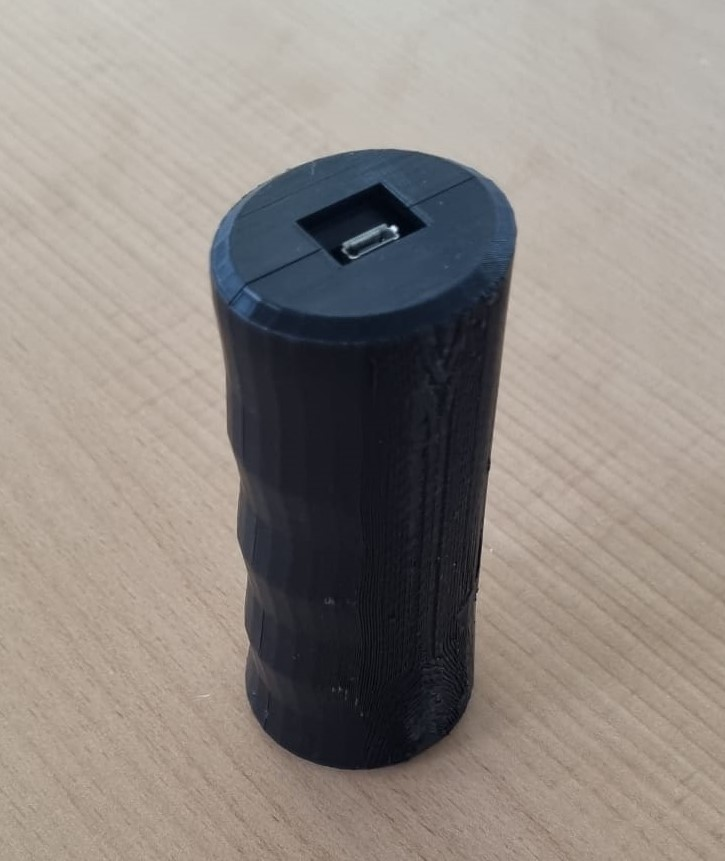
\includegraphics[width=0.8\linewidth]{content/images/3DPrint_closed.jpeg}
      \caption{3D Druck geschlossen}
    \end{center}
  \end{figure}
\end{minipage}
